\chapter{Data Selection}

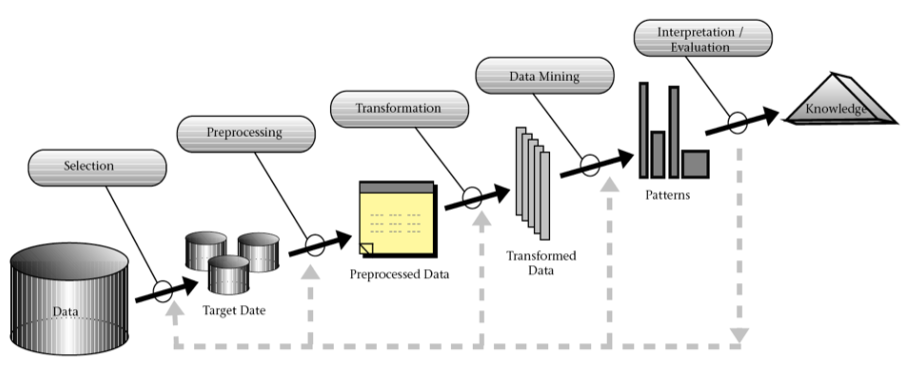
\includegraphics[width=\textwidth]{images/DM_Process.png}

\begin{itemize}
	\item Selection: 
	\begin{itemize}
		\item What data is available?
		\item What do I know about the provenance of the data?
		\item What do I know about the quality of the data?
	\end{itemize}
	\item Exploration
	\begin{itemize}
		\item Get an intitial understanding of the data
		\item Calculate basic summarization statistics
		\item Visualize the data
		\item Identify data problems such as outliers, missing values, duplicate records
	\end{itemize}
\end{itemize}

\chapter{Preprocessing and Transformation}
\begin{itemize}
\item Transform data into a representation that is suitable for the chosen data mining methods
\begin{itemize}
\item number of dimensions
\item scales of attributes (nominal, ordinal, numeric)
\item amount of data (determines hardware requirements)
\end{itemize}
\item Methods
\begin{itemize}
\item Aggregation, sampling
\item Dimensionality reduction / feature subset selection
\item Attribute transformation / text to term vector
\item Discretization and binarization
\end{itemize}
\item Good data preparation is key to producing valid and reliable models
\item Data preparation estimated to take 70-80\% of the time and effort of a data mining project!
\end{itemize}

\chapter{Data Mining}
\begin{itemize}
\item Input: Preprocessed Data
\item Output: Model / Patterns
\end{itemize}

\begin{enumerate}
\item Apply data mining method
\item Evaluate resulting model / patterns
\item Iterate:
\begin{itemize}
\item Experiment with different parameter settings
\item Experiment with different alternative methods – Improve preprocessing and feature generation – Combine different methods
\end{itemize}
\end{enumerate}

\chapter{Interpretation / Evaluation}
\begin{itemize}
	\item Output of Data Mining
	\begin{itemize}
		\item Patterns
		\item Models
	\end{itemize}
	\item In the end, we want to derive value from that, e.g.,
	\begin{itemize}
		\item gain knowledge
		\item make better decisions
		\item increase revenue
	\end{itemize}
\end{itemize}



